\documentclass[10pt,a4paper]{report}
\usepackage[latin1]{inputenc}
\usepackage{amsmath}
\usepackage{amsfonts}
\usepackage{amssymb}
\usepackage{graphicx}
\usepackage{hyperref}
\usepackage{multicol}
\usepackage[margin=0.1 in]{geometry}
\usepackage{tikz}
\usepackage{romannum}
\usepackage{listings}
\usetikzlibrary{arrows,shapes.gates.logic.US,shapes.gates.logic.IEC,calc}
\usepackage{titlesec}
\titlespacing{\subsection}{1pt}{\parskip}{3pt}
\titlespacing{\subsubsection}{0pt}{\parskip}{-\parskip}
\titlespacing{\paragraph}{0pt}{\parskip}{\parskip}
\newcommand{\myvec}[1]{\ensuremath{\begin{pmatrix}#1\end{pmatrix}}}
\let\vec\mathbf

\begin{document}

\centering {
\includegraphics[scale=0.07]{IITH.png}} \vspace{3mm}\\ \raggedleft Name:T.Manasa Reddy\vspace{2mm}\\ \raggedleft Roll No.: FWC22048\vspace{2mm}\\ \raggedright Sep 2022 \hspace{12cm} \raggedleft manasatanuboddi@gmail.com \vspace{10mm}
\\ \centering \Large \textbf{MATRIX ASSIGNMENT} \normalsize \vspace{15mm}

\begin{multicols}{2}
\section{Problem:}  Construct a triangle ABC in which BC=7cm, $\angle{B}=75^0$ and AB + AC = 13 cm.\vspace{3mm}
\section{Solution}
The input parameters for this construction are
\begin{center}
\begin{tabular}{|c|c|c|}
	\hline
	\textbf{Symbol}&\textbf{Value}&\textbf{Description}\\
	\hline
	BC & a & where a is 7cm\\
	\hline
	AB & b & AB distance is b \\
	\hline 
	AC & c & AC distance is c \\
	\hline
	$\angle{BC}$ & $75^0$ &  $\Delta$ABC \\
	\hline
	$\vec{C}$ & $\myvec{a\\0}$ & BC length is equal to a\\
	\hline
	$\vec{A}$ & $\myvec{ cos\theta \\ sin\theta}$ & using the cosine formula in $\Delta$ABC\\
	\hline
\end{tabular}
\end{center}
\raggedright {termux commands :}
\begin{center}
\fbox{\parbox{8.5cm}{bash line.sh.........using shell command}}
\end{center}
\raggedright\textbf{Caluclating Other Coordinate: } \\
\raggedright Let the coordinates of A are $X_{2}$,$Y_{2}$ respectively. \\
  \raggedright Let \textbf{A} =
  $\begin{pmatrix} 
 \cos \theta\\
  \sin\theta \\
\end{pmatrix}$ \\
\raggedright Using the Cosine formula in  $\Delta$ABC, \\ \vspace{3mm}
\begin{equation}
{b}^2\hspace{1.5cm}= {a}^2 + {c}^2 - 2accos\vec{B}
\end{equation}
\begin{equation}
(b+c)(b-c) = {a}^2- 2 \times a \times ccos\vec{B}
\end{equation}
\begin{equation}
K(b-c) = {a}^2- 2 \times a \times ccos\vec{B}
\end{equation}
\begin{equation}
bk-ck+2\times a\times c\times cos\vec{B} = a^2
\end{equation}
\begin{equation}
bk-c(k+2acos\vec{B})=a^2
\end{equation}
\raggedright  From the above we know that:-
\begin{equation}
        b+c=13 
\end{equation}\\
     From the above, we obtain the matrix equation:- \\ \vspace{3mm}
        $\begin{pmatrix}
            k & -k+2acos\vec{B}\\
            1 & 1  \\
        \end{pmatrix}$% 
        $\begin{pmatrix}
            b \\
            c \\
        \end{pmatrix}$% 
           =
           $\begin{pmatrix}
            a^2\\
            k\\
        \end{pmatrix}$%   
        \vspace{5mm}           
   \\  
   reduced row echelon form of \left \begin{pmatrix}13 & -13 + \frac{\sqrt{2} \left(-7 + 7 \sqrt{3}\right)}{2} & 49\\1 & 1 & 13\end{pmatrix}\right
        \vspace{3mm}
        \\Divide row1 by 13: R1 = $\frac{R1}{13}$
        \vspace{7mm}
        \\ \left $\begin{pmatrix} 1 & -\frac{ -7\sqrt{6} \left + 7 \sqrt{2} + 26 \right)}{26} & \frac{49}{13}\\ 1& 1 & 13\end{pmatrix}\right \vspace{5mm}
        \\ Subtract row 1 from row 2: R2 = R2 - R1 \vspace{3mm}
        \\\left $\begin{pmatrix}1 & -\frac{ -7\sqrt{6} \left + 7 \sqrt{2} + 26 \right)}{26} & \frac{49}{13}\\ 0 & -\frac{ -7\sqrt{6} \left + 7 \sqrt{2} + 52 \right)}{26} & \frac{120}{13}\end{pmatrix}\right \vspace{6mm}
        \\ Multiply row 2 by $\frac{26}{- 7 \sqrt{6} + 7 \sqrt{2} + 52}$:\vspace{3mm}
         R2=$\frac{26}{- 7 \sqrt{6} + 7 \sqrt{2} + 52}$  
         \vspace{6mm}
    \\ Add row 2 multiplied by $\frac{- 7 \sqrt{6} + 7 \sqrt{2} + 26}{26}$ \vspace{5mm}
     \\ \left $\begin{pmatrix}1 & 0 &-\frac{ 91\sqrt{6} \left + 91\sqrt{2} + 436\right)}{-7\sqrt{6} \left + 7 \sqrt{2} + 52 \right)}\\ 0 & 1 &\frac{240}{ -7\sqrt{6} + 7 \sqrt{2} + 52} \end{pmatrix}\right  \vspace{5mm}
     \\ $\begin{pmatrix}
     b \\
     c \\
     \end{pmatrix}$%
     = $\begin{pmatrix}
     -\frac{ 91\sqrt{6} \left + 91\sqrt{2} + 436\right)}{-7\sqrt{6} \left + 7 \sqrt{2} + 52 \right)} \\
     \frac{240}{ -7\sqrt{6} + 7 \sqrt{2} + 52}
     \end{pmatrix}$%
     \vspace{5mm}
    \\ \raggedright \textbf{A} = c$\begin{pmatrix}
                 cos 75 \\ 
                 sin 75 \\
              \end{pmatrix}$%
              =$\begin{pmatrix}
                 1.33 \\
                 5.15 \\
                 \end{pmatrix}$%
                 \vspace{5mm}
              \\ \raggedright  \textbf{B} = $\begin{pmatrix}
                 0\\
                 0\\
              \end{pmatrix}$% 
              \vspace{5mm}
             \\ \raggedright  \textbf{C} = $\begin{pmatrix}
                  7\\
                  0\\
              \end{pmatrix}$%
              \vspace{5mm}
\\
Below python code realizes the above construction : 
\fbox{\parbox{8.5cm}{\url{https://github.com/manasareddy442002/fwc-moudle1/blob/matrix-lines/matrix.py}}}

 \section{Construction}
 	\begin{center}
  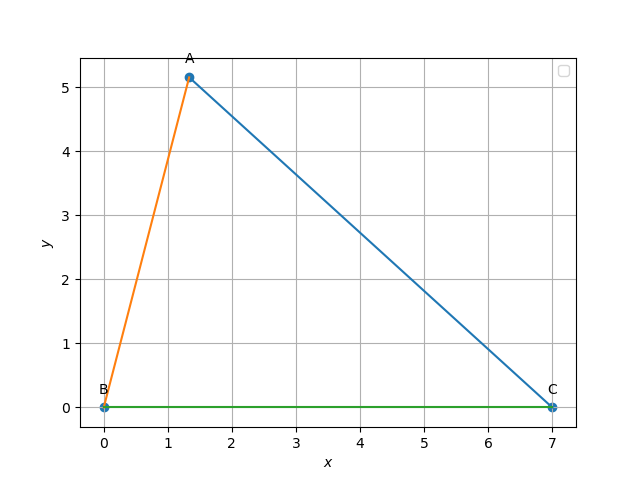
\includegraphics[scale=0.5]{Figure_1.png}
  	\end{center}
\vspace{3cm}
\end{multicols}

\end{document}
